\documentclass[11pt,a4paper]{article}

\usepackage[T1]{fontenc}
\usepackage{mathpazo}
\usepackage[utf8]{inputenc}
\usepackage[english]{babel}
\usepackage[margin=2.6cm]{geometry}
\usepackage[expansion=false]{microtype}
\usepackage{booktabs}
\usepackage{array}
\usepackage{xcolor}
\usepackage{pgfplots}
\pgfplotsset{compat=1.16}
\usepackage{setspace}
\usepackage{enumitem}
\usepackage[hidelinks]{hyperref}
\usepackage{caption}

\definecolor{accent}{HTML}{0B6E6E}
\definecolor{muted}{HTML}{6B7280}

\newcommand{\paperauthor}{Leonardo Covarrubias Garc\'ia}
\setstretch{1.08}
\emergencystretch=2em
\setlength{\parskip}{0.55em}
\setlength{\parindent}{0pt}
\captionsetup{font=small,labelfont=bf}

\title{\textbf{From Meter to Meaning}\\[0.3em]
\large A Reading of the \emph{State of Tokenomics 2026} Report}
\author{\paperauthor\\[0.35em]
  {\normalsize\color{muted}AI-Native Economist}}
\date{October 2026}

\begin{document}
\maketitle

\begin{abstract}
\noindent
The Tokenomics Foundation's inaugural \emph{State of Tokenomics} report (Release Candidate 1.0, 23 September 2026) draws on 472 responses from large enterprises across 11 industries. Read next to the FinOps Foundation's argument that Tokenomics and FinOps for AI are two projections of one body of work, its data tells a coherent story. Organizations now consume AI through many models in many places, and most can see a fair part of what they spend. Yet roughly three in four cannot confidently show a business outcome to the CFO, and the single largest challenge respondents name is proving value, not paying less. This text argues that the unit of account has outrun the unit of value: the field's difficulty has migrated from measuring consumption to measuring consequence. It closes with five practice principles and a candid account of the report's own data inconsistencies.
\end{abstract}

\section{Introduction}

A kilowatt hour is how electricity is metered; it is not what electricity is for. The same holds for the token. It is the instrument by which the output of an AI system is counted and billed, and a discipline built only around reading that instrument would resemble a civilization that mistook the thermometer for the weather.

This text is a reading of a survey, not a survey. It is \emph{not} original primary research. It interprets the \emph{State of Tokenomics} report published by the Tokenomics Foundation, a Linux Foundation project, and places it beside a recent piece of FinOps Foundation commentary on how Tokenomics and FinOps for AI relate. The aim is modest and specific: to extract what the data supports, to mark what it does not, and to translate both into a short set of principles for teams that must decide how to spend on AI today.

A note on attribution. The report is authored by the Tokenomics Foundation (tokeneconomics.com). The FinOps Foundation links to it from its own site and has published commentary on the relationship between the two disciplines, but it is not the report's author.

\section{The source and its limits}

The report describes 472 responses across 11 industries, representing approximately \$4.6 trillion in revenue across nearly 500 companies, with a median respondent revenue of \$1.8 billion. Technology and software account for 40\% of respondents, financial services for 17\%, and professional services for 11\%. This is a population of large organizations, weighted toward technology, and every conclusion below inherits that tilt.

Two cautions frame the reading. First, the version analyzed is labelled a Release Candidate, and several of its figures do not reconcile with one another; Section~\ref{sec:limits} lists them. Second, the report is a perception survey. Its measures, such as confidence in spend visibility, are self-reported judgments, not audited quantities. Where the report states a correlation, this text repeats it as a correlation and does not promote it to a cause.

\section{Tokenomics is not token counting}

The FinOps Foundation's commentary by Mike Fuller makes a distinction worth preserving, because the rest of the data is easier to read with it in hand~\cite{fuller2026}. The common misreading takes Tokenomics to mean tracking cost per token. Fuller's correction is that the token sits at the end of a production chain that runs from energy and capital through silicon, serving infrastructure, model selection and application design, and then onward into packaging, pricing and margin. Tokenomics, on this account, is the economics of the entire chain, and counting tokens is its least interesting part.

The commentary then offers an image: Tokenomics and FinOps for AI are two projections of the same object taken along different axes. FinOps for AI collapses breadth of subject in order to render depth of practice, namely allocation, forecasting, ownership and operating cadence. Tokenomics collapses depth of practice in order to render breadth of subject, from power to price. Neither is a subset of the other, and they do not compete. A concrete case makes the point. When the price of AI capacity rises, FinOps may correctly report an alarming overrun, while Tokenomics may equally correctly report that tokens consumed per resolved outcome have been falling. The decisive finding, that a well-run system is absorbing a market shock, lives only in the space between the two reports.

This is the lens applied below. When the survey shows a gap, the useful question is which projection is missing from the room.

\section{What the data shows}

\subsection{Cardinality: many models in many places}

The report finds that AI consumption has become plural along every axis (Table~\ref{tab:surfaces}). Nearly all respondents (96\%) use a model provider directly, 87\% consume tokens through a cloud provider, and 64\% use AI embedded in other products. A further 32\% run edge, local or desktop models, 31\% rent hardware, and 29\% operate private hardware. Half of AI consumers spread across four of these six channels, and nearly one in five already use at least one of Deepseek, Qwen, Kimi or GLM.

\begin{table}[h]
\centering
\small
\begin{tabular}{@{}lr@{}}
\toprule
Consumption channel & Respondents using it \\
\midrule
Model provider (direct) & 96\% \\
Token provider (cloud) & 87\% \\
Embedded AI & 64\% \\
Edge, local, desktop & 32\% \\
Rented hardware & 31\% \\
Private hardware & 29\% \\
\bottomrule
\end{tabular}
\caption{Share of respondents using each procurement or hosting channel. Source: \emph{State of Tokenomics}, RC 1.0.}
\label{tab:surfaces}
\end{table}

The mix of model types is also shifting in the respondents' own expectations. Today, 51\% describe their workloads as heavily frontier (8 to 10 on the report's 10-point self-assessment), while only 24\% expect to sit there in twelve months. The heaviest frontier users plan the largest shift: those at 10 today expect to move down by an average of 2.7 points, and only 17\% anticipate moving toward more frontier usage. These are stated intentions, not observed behavior, so the direction is informative but the magnitudes should be held loosely.

The implication for economics is direct. A cost model that assumes one vendor and one price list describes a minority of these organizations. High cardinality means that attribution, normalization and comparison become the precondition of any serious analysis.

\subsection{Visibility is not value}

The report's most arresting contrast sits between two questions. Asked how confident they are in their visibility into AI spend, respondents answer with moderation: 20\% not confident, 28\% slightly, 39\% moderately and 14\% very confident. Asked how confident they are in proving AI business outcomes to the CFO, the picture darkens: 39\% not confident, 34\% slightly, 17\% moderately and 9\% very (Table~\ref{tab:confidence}). Roughly three in four therefore cannot confidently demonstrate value.

\begin{table}[h]
\centering
\small
\begin{tabular}{@{}lrr@{}}
\toprule
Confidence level & In spend visibility & In proving outcomes to the CFO \\
\midrule
Not confident & 20\% & 39\% \\
Slightly confident & 28\% & 34\% \\
Moderately confident & 39\% & 17\% \\
Very confident & 14\% & 9\% \\
\bottomrule
\end{tabular}
\caption{Self-reported confidence. Columns may not sum to 100\% because of rounding in the source.}
\label{tab:confidence}
\end{table}

The report notes that higher visibility generally correlates with better value confidence, and that the very confident share traits in common: spend that is metered and attributable across workloads and teams, and tracking of concrete business output metrics such as tickets, pull requests or revenue. Confidence also appears to vary by company size, with smaller organizations more likely to see the whole picture, though the slide stating this does not define its metric (see Section~\ref{sec:limits}).

Philosophically, this is the old distinction between knowing a thing's quantity and knowing its worth. Seeing a bill precisely does not tell you whether the thing bought was good. The data suggests that many organizations have solved the first problem partially and have barely begun the second.

\subsection{The binding constraint is meaning, not price}

When asked to name their biggest Tokenomics challenge, 43\% of respondents say proving value or ROI, the largest single answer, followed by visibility and attribution of spend (27\%) and measurement and data quality (18\%). Only 7\% name cost or pricing complexity (Figure~\ref{fig:challenges}).

\begin{figure}[h]
\centering
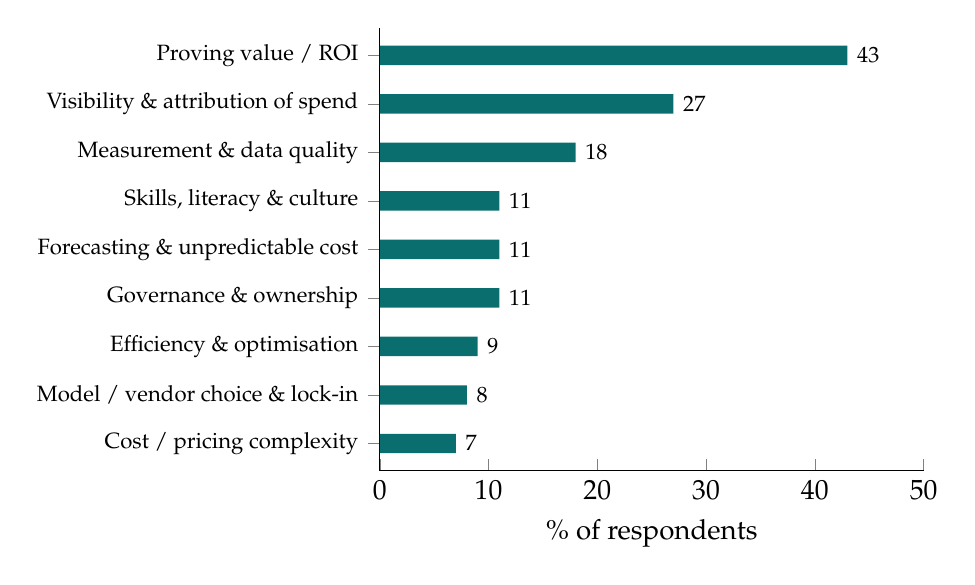
\begin{tikzpicture}
\begin{axis}[
  xbar, bar width=7pt,
  width=0.7\textwidth, height=7.2cm,
  xmin=0, xmax=50,
  xlabel={\% of respondents},
  symbolic y coords={
    {Cost / pricing complexity},
    {Model / vendor choice \& lock-in},
    {Efficiency \& optimisation},
    {Governance \& ownership},
    {Forecasting \& unpredictable cost},
    {Skills, literacy \& culture},
    {Measurement \& data quality},
    {Visibility \& attribution of spend},
    {Proving value / ROI}},
  ytick=data,
  y tick label style={font=\footnotesize},
  nodes near coords,
  nodes near coords style={font=\footnotesize},
  axis x line*=bottom, axis y line*=left,
  enlarge y limits=0.07,
]
\addplot[fill=accent, draw=none] coordinates {
  (7,{Cost / pricing complexity})
  (8,{Model / vendor choice \& lock-in})
  (9,{Efficiency \& optimisation})
  (11,{Governance \& ownership})
  (11,{Forecasting \& unpredictable cost})
  (11,{Skills, literacy \& culture})
  (18,{Measurement \& data quality})
  (27,{Visibility \& attribution of spend})
  (43,{Proving value / ROI})};
\end{axis}
\end{tikzpicture}
\caption{Biggest Tokenomics challenges named by respondents. Source: \emph{State of Tokenomics}, RC 1.0.}
\label{fig:challenges}
\end{figure}

The same orientation appears in what respondents ask of their providers. Their top requests are more transparency and granular data (23\%), standards such as FOCUS (19\%), and attribution and tagging (17\%). The request for cheaper prices comes last, at 4\%. Buyers, in other words, are asking for better instruments of judgment before they ask for lower prices. The conventional picture of an AI buyer haggling over the rate card does not match this sample.

\subsection{Ownership and routing travel with value}

Two organizational facts correlate strongly with the ability to show value. The first is ownership. In the report, 88\% of organizations have a defined owner for AI economics and 12\% have none; none of the latter can connect AI spend to a CFO-level outcome. Ownership sits most often with technology leadership (35\%, CTO, CIO or technology), then shared across functions (26\%), followed by an executive or the CEO (9\%), other (7\%), AI leadership (6\%) and finance (5\%). Those with defined ownership are reported as 3.7 times more likely to show value to the CFO.

The second is model routing. About 86\% are evaluating or using a model router, and those using routers are reported as four times more likely to show CFO value. Routing is also sought across company sizes, whether bought, built in-house or both.

Two readings of these correlations deserve to be held at once. The optimistic reading is that ownership and routing are levers: appoint an owner, route workloads to the right model, and value becomes provable. The skeptical reading is that organizations capable of defining ownership and deploying routers are already the more mature ones, and maturity, not the levers, produces the outcome. The report does not separate the two, and neither does this text. What can be said is that both are practical, low-regret organizational moves, which is a reasonable argument for acting on them while remaining honest about the evidence.

It is worth observing, in the spirit of the projection argument, that the owner is rarely finance. Only 5\% of respondents place AI economics there. The question FinOps is built to ask, whose budget is this and did it close, is being answered inside technology functions more often than inside the function traditionally trained to ask it.

\subsection{Beyond the bill: pricing, energy and labor}

The report also records that the economics of AI reach well past infrastructure. Some 52\% of companies have changed or are considering changes to their own pricing, 30\% report no change and 18\% say it is too early to tell; the accompanying commentary points toward usage-based and outcome-based models and toward pressure on margins from unpredictable AI cost. Another 38\% consider energy consumption in their Tokenomics, typically those who own or rent hardware and who train first-party models or use open-weight models.

On labor, the report offers qualitative themes rather than counts: productivity gains from existing staff, workforce reductions attributed to AI in some firms, budget moved from hiring toward AI as a staffing alternative, and a shift toward AI-specialized roles and away from entry-level positions. Because no proportions are given, none are inferred here. The qualitative signal is nonetheless relevant: it is the far end of the chain described in Section~3, where the economics of tokens meets the economics of people.

\section{Five practice principles}

The following principles are this reading's own synthesis. They are interpretations of the report and the commentary, not claims made by either.

\begin{enumerate}[leftmargin=1.6em, itemsep=0.2em]
\item \textbf{Treat the token as an instrument, not an objective.} Cost per token is a meter reading. Define cost per outcome (a resolved ticket, a merged pull request, a closed case) and judge systems by that.
\item \textbf{Instrument attribution before optimization.} The very confident share spend that is metered and attributable across workloads and teams. Optimizing what cannot be attributed produces savings no one can claim.
\item \textbf{Name an owner, and name one on purpose.} Defined ownership accompanies a markedly higher ability to show value. Shared ownership is common and viable, but it should be a decision and not a default.
\item \textbf{Adopt shared data standards early.} With many models in many places, and buyers asking providers for standards such as FOCUS, normalization is infrastructure. Building custom correlation tooling on top of incompatible formats is a recurring cost.
\item \textbf{Hold both projections.} Let FinOps for AI ask the budget question, drive ownership and close the loop. Let Tokenomics evaluate whether quality holds as consumption falls, and decide what the output should sell for. Read the space between their reports as a finding.
\end{enumerate}

\section{Limitations and methodological note}
\label{sec:limits}

This text is a reading of a published report and of a piece of commentary. It contains no original primary data, and it draws on no client, employer or production cost data. Every figure is cited indirectly from the sources listed in the references. The report is a Release Candidate and may change before final publication. In preparing this reading, the following issues in the source were noted, and the analysis above avoids relying on the affected figures.

\begin{itemize}[leftmargin=1.4em, itemsep=0.2em]
\item \textbf{Revenue totals do not reconcile.} The per-industry revenue figures shown for the 11 industries sum to roughly \$8.5 trillion, while the headline states \$4.6 trillion. A reported mean revenue of about \$21 billion across 472 respondents would imply roughly \$9.9 trillion. The \$4.6 trillion headline is quoted as reported but should be treated with caution; only the response count and the median (\$1.8 billion) are relied on as descriptive context.
\item \textbf{An apparent tension in the confidence statistics.} The report states that 60\% of organizations with moderately confident spend visibility are unable to provide a measurable outcome to the CFO, while 25\% of those with highly confident spend are able to. Read literally, the second figure is lower than the complement of the first (40\%), which would contradict the claim that higher visibility correlates with better value confidence. The phrasing may be imprecise, so this text does not use the 25\% figure.
\item \textbf{An undefined metric by company size.} The slide stating that confidence falls as revenue rises lists \$10B+ at 23\%, above the \$1B to \$10B (17\%) and \$100M to \$1B (14\%) bands, and does not state which confidence is being measured. The trend is therefore not monotonic and is cited here only in general terms.
\item \textbf{Sample composition.} The sample is large-enterprise and technology-weighted. Results should not be generalized to small organizations or to regions and sectors that are thinly represented.
\item \textbf{Self-report and correlation.} The ``3.7x'' and ``4x'' associations are correlations among self-reported answers. They are not evidence that ownership or routing causes value.
\end{itemize}

\section{Conclusion}

The report's central lesson is easy to state and hard to practice. The industry has learned, impressively quickly, to count what AI consumes. It has not yet learned, in most organizations, to say what that consumption was worth. The meter is nearly installed; the meaning is not. Reading Tokenomics and FinOps for AI as two projections of one object offers a practical discipline for the gap: let each ask the question the other cannot see, and insist that every question worth asking reaches a decision that can answer it.

\begin{thebibliography}{9}\small
\bibitem{tokenomics2026} Tokenomics Foundation. \emph{State of Tokenomics}, Release Candidate 1.0, 23 September 2026. \url{https://www.tokeneconomics.com/state-of-tokenomics/}
\bibitem{fuller2026} Fuller, M. ``FinOps and Tokenomics: How do they fit together?'' FinOps Foundation Insights, 25 August 2026. \url{https://www.finops.org/insights/finops-tokenomics-fit-together/}
\end{thebibliography}

\vfill
\begin{center}
\footnotesize\color{muted}
This text is an independent reading. It is not affiliated with, or endorsed by, the Tokenomics Foundation or the FinOps Foundation.
\end{center}

\end{document}
